\documentclass[]{article}
\usepackage{float}
\usepackage{graphicx}
\usepackage[]{subcaption}
\captionsetup[figure]{labelfont={bf,footnotesize},textfont=footnotesize}
\captionsetup[table]{labelfont={bf,footnotesize},textfont=footnotesize}
\usepackage{xcolor}
\usepackage{listings}
\lstset{
  frame=single,
  breaklines=true,
  postbreak=\raisebox{0ex}[0ex][0ex]{\ensuremath{\color{red}\hookrightarrow\space}}
}
\usepackage{hyperref}
\usepackage[]{amsmath}

\newcommand{\TwoRowCell}[2][c]{%
\begin{tabular}[#1]{@{}c@{}}#2\end{tabular}}

\title{Simulation - Assignment 2}
\author{Anton Roth}
\date{\today}

\begin{document}
\begin{titlepage}
  \maketitle
  \thispagestyle{empty}
\end{titlepage}

\section*{Introduction}
All tasks have been solely implemented in {\it Matlab}. Files \textit{task1.m} and \textit{task2.m} contain the implementation where each sub-task are clearly separated with a lot of \textit{\#}.

\section*{Task 1}

\subsection*{1.a - Problem formulation}
\label{sec:1a}
\begin{align*}
  \text{Number of packages (in 1000s) of each type: } & x_i,\ i = 1, 2, 3, 4, 5 \\
  \text{Maximise: } & Z = 4x_1+3x_2+2x_3+2x_4+x_5 \\
  \text{Demand limitations: } & x_1 \leq 16 \\
  & x_3 \leq 2 \\
  & x_1+x_2+ x_3 \leq 34 \\
  & x_4+ x_5 \leq 28 \\
  \text{Capacity limitations: } & 2x_1 \leq 36 \\
  & 2x_2+2x_3+2x_4+x_5 \leq 216 \\
  & 0.1x_1+x_2+0.5x_4 \leq 18 \\
  \text{Lower bound: } & x_i \geq 0 \\
  \label{al:task1a}
\end{align*}

%Get shadow prices with Matlab:
%\url{http://fr.mathworks.com/matlabcentral/newsreader/view_thread/160654}

\subsection*{1.b - Problem solution}
The problem formulation was translated into the matrix form used by the function \textit{linprog}. The \textit{dual-simplex} algorithm was chosen. The solution is as follows:
\begin{align*}
  & x^T = [16, 14.8, 2, 0, 28] \\
  & Z = 140.4
\end{align*}
I.e. UniCam's profit is maximised when 16000 packages of type \textbf{I}, 14800 packages of type \textbf{II}, 2000 packages of type \textbf{III}, 0 packages of type \textbf{IV} and 28000 packages of type \textbf{V} is sold.
The total profit in this case is $1,404,000,000$ SEK.

\subsection*{1.c - Shadow prices}
The shadow prices for all constraints, i.e. the profit that can be made with an incrementation of the constraint by one unit, can easily be determined with the Lagrange multipliers given by Matlabs \textit{linprog} function.
All shadow prices, denoted $S$, are presented below in the order as the constraints are introduced in section \ref{sec:1a}:
\begin{align*}
  S = [3.4, 2, 0, 1, 0, 0, 3]
\end{align*}
A conclusion that can be made from this is that the by adjusting the first constraint, i.e. $x_1 \leq 16$ (demand of package \textbf{I} is at maximum 16 000), the largest possible increase in the optimised profit ($34,000,000$ per thousand units of package \textbf{I}) can be made.

\subsection*{1.d - ``Allowable increase''}
The dependence of the maximum demand of package \textbf{III} and the optimised maximal profit is presented in Figure \ref{fig:task1d}.

\begin{figure}[H]
  \centering
  \includegraphics[width=\textwidth]{../task1d.pdf}
  \caption{The maximum demand of package \textbf{III} is plotted against the optimised maximal profit (left y-axis) in blue. The shadow price for the increased maximum demand of package \textbf{III} is presented on the right y-axis in red.}
  \label{fig:task1d}
\end{figure}

The optimised maximal profit flattens after 26 iterations, i.e. when the maximum demand of the package is 17600.
From Figure \ref{fig:task1d} it is clear that the shadow price changes twice, first from 2 to 1 and then from 1 to 0.
Of course, if the shadow price is 0, no increase in the total profit is observed.
A conclusion one can draw is that for a demand of package \textbf{III} above 17600 the total profit for UniCAM cannot be increased (for the current situation).

\subsection*{1.e - Price variations}
The code was implemented after the hint and the results were the following:
\begin{equation*}
  0.6 \leq \text{Price of package \textbf{I}} \leq \infty
  \label{eq:task1e}
\end{equation*}
It was concluded that the upper limit must be $\infty$ since the optimal solution did not change even though the price was huge.

The optimal solution is very robust to changes in the price of package \textbf{I} and this is reasonable I think since the profit from this package is the largest with some margin (cf. $4*16 = 64$ for package \textbf{I} and $1*28 = 28$ for package V which has the second largest profit).
The reason why the upper limit is $\infty$ is because the coefficient in the objective function is the largest for parameter 1, which corresponds to the price of package \textbf{I}, cause you will always gain the most profit by increasing the price.

\section*{Task 2}

\subsection*{2.a - Problem solution}
The integer problem was solved with the function \textit{intlinprog} and the following was the result:
\begin{equation}
  x_1 = 3, \ x_2 = 2 \ \& \ z = 13
  \label{eq:task2a}
\end{equation}

\subsection*{2.b - LP and rounding}
The relaxed integer problem was solved with \textit{linprog} with the following result:
\begin{equation}
  x_1 = 1.6, \ x_2 = 2.6 \ \& \ z = 14.6
  \label{eq:task2b}
\end{equation}

The obtained parameter of the relaxed problem was rounded up/down and the paired together in all possible four combinations.
The value of the objective function was calculated for each combination and all constraints were checked.
The result is presented in Table \ref{tab:task2b}.
\begin{table}[H]
  \centering
  \caption{Value of objective function for each combination of rounded parameter solutions. In the last column it is also noted of which constraint that is violated, if that is the case.}
  \label{tab:task2b}
  %\resizebox{\textwidth}{!}{% Important that this only covers the tabular!
  \begin{tabular}{|c|c|c|c|}
  \hline
  {\bf $x_1$ } & {\bf $x_2$ } & {\bf $z$} & \TwoRowCell{\bf Constraint \\ \bf violated} \\ \hline
  1  & 2                                  & 11                      &  -                         \\ \hline
  2  & 2                                 & 12                    & -                       \\ \hline
  1  & 3                                 & 16                  &  first                    \\ \hline
  2  & 3                                 & 17                   & third                    \\ \hline
  \end{tabular}%
%}
\end{table}

Clear from Table \ref{tab:task2b} is that the optimal integer solution is not found with rounding the relaxed problem.

\subsection*{2.c - Branch and Bound Method}
The result of the branch and bound method is presented with Figure \ref{fig:task2c}.

\begin{figure}[H]
  \centering
  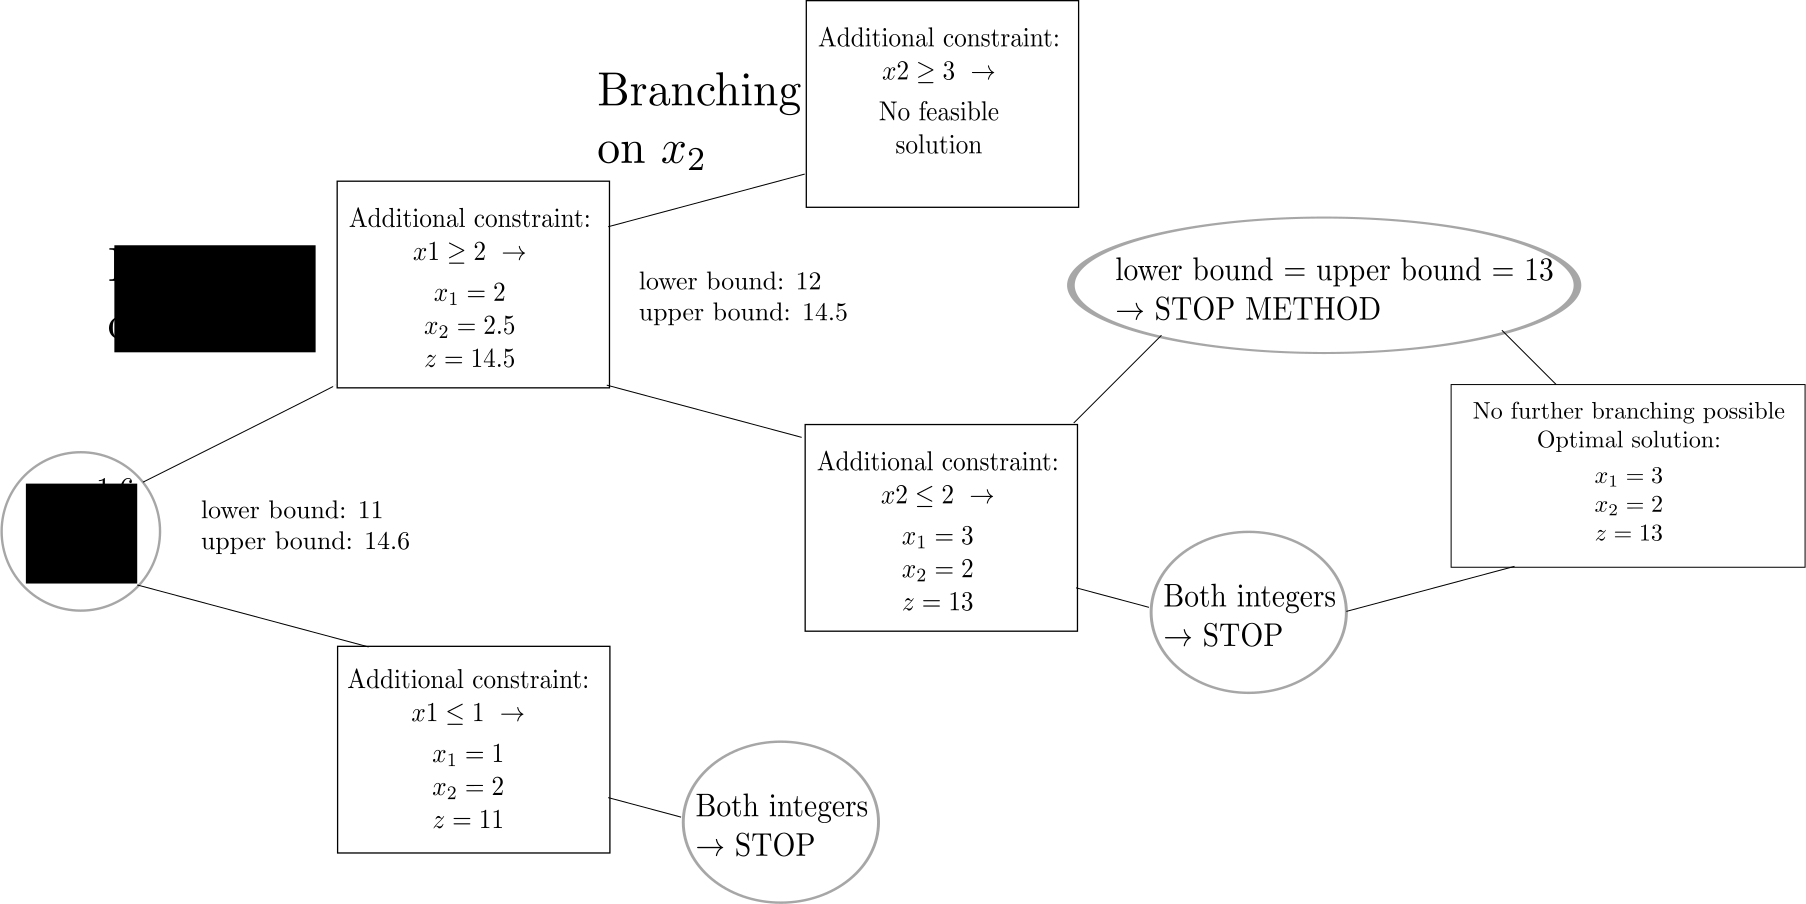
\includegraphics[width=\textwidth]{../b2b_tree.png}
  \caption{Branch and bound method tree for the relaxed integer problem. }
  \label{fig:task2c}
\end{figure}

A branch is cut either if there is no feasible solution or both solution parameters are integers. The process is stopped when the upper bound is less than or equal to the upper bound and/or when no further branching is possible (this ocurred simultaneously for the above example).


\end{document}

